%label:"fig:polterovichSurgery"
%author:JeffHicks
%name:"Polterovich Surgery"
%type:"figure"
%parent:"prp:polterovichSurgery"
%caption:"The connect sum of two Lagrangian curves in a surface"


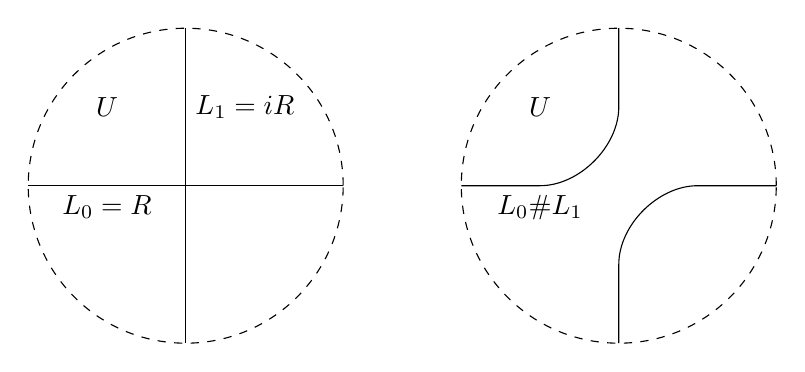
\begin{tikzpicture}
      \draw[dashed]  (0,0) circle[radius=2];
      \draw (-2,0) -- (2,0) (0,2) -- (0,-2);
      \node at (-1,1) {$U$};
      \node[right] at (0,1) {$L_1=i\mathbb R$};
      \node[below] at (-1,0) {$L_0=\mathbb R$};\begin{scope}[shift={(5.5,0)}]

      \draw[dashed]  (0,0) circle[radius=2];
      \node at (-1,1) {$U$};
      
      \node[below] at (-1,0) {$L_0\#L_1$};
      
      \draw (-2,0) .. controls (-1.5,0) and (-1.5,0) .. (-1,0) .. controls (-0.5,0) and (0,0.5) .. (0,1) .. controls (0,1.5) and (0,1.5) .. (0,2) ;
      \draw (2,0) .. controls (1.5,0) and (1.5,0) .. (1,0) .. controls (0.5,0) and (0,-0.5) .. (0,-1) .. controls (0,-1.5) and (0,-1.5) .. (0,-2);
\end{scope}
      
\end{tikzpicture}
